
%% bare_conf.tex
%% V1.3
%% 2007/01/11
%% by Michael Shell
%% See:
%% http://www.michaelshell.org/
%% for current contact information.
%%
%% This is a skeleton file demonstrating the use of IEEEtran.cls
%% (requires IEEEtran.cls version 1.7 or later) with an IEEE conference paper.
%%
%% Support sites:
%% http://www.michaelshell.org/tex/ieeetran/
%% http://www.ctan.org/tex-archive/macros/latex/contrib/IEEEtran/
%% and
%% http://www.ieee.org/

%%*************************************************************************
%% Legal Notice:
%% This code is offered as-is without any warranty either expressed or
%% implied; without even the implied warranty of MERCHANTABILITY or
%% FITNESS FOR A PARTICULAR PURPOSE!
%% User assumes all risk.
%% In no event shall IEEE or any contributor to this code be liable for
%% any damages or losses, including, but not limited to, incidental,
%% consequential, or any other damages, resulting from the use or misuse
%% of any information contained here.
%%
%% All comments are the opinions of their respective authors and are not
%% necessarily endorsed by the IEEE.
%%
%% This work is distributed under the LaTeX Project Public License (LPPL)
%% ( http://www.latex-project.org/ ) version 1.3, and may be freely used,
%% distributed and modified. A copy of the LPPL, version 1.3, is included
%% in the base LaTeX documentation of all distributions of LaTeX released
%% 2003/12/01 or later.
%% Retain all contribution notices and credits.
%% ** Modified files should be clearly indicated as such, including  **
%% ** renaming them and changing author support contact information. **
%%
%% File list of work: IEEEtran.cls, IEEEtran_HOWTO.pdf, bare_adv.tex,
%%                    bare_conf.tex, bare_jrnl.tex, bare_jrnl_compsoc.tex
%%*************************************************************************

% *** Authors should verify (and, if needed, correct) their LaTeX system  ***
% *** with the testflow diagnostic prior to trusting their LaTeX platform ***
% *** with production work. IEEE's font choices can trigger bugs that do  ***
% *** not appear when using other class files.                            ***
% The testflow support page is at:
% http://www.michaelshell.org/tex/testflow/


%
\documentclass[conference]{IEEEtran}
\usepackage{cite}
\ifCLASSINFOpdf
  \usepackage[pdftex]{graphicx}
\fi
\usepackage[cmex10]{amsmath}
\usepackage{algorithmic}
\usepackage{array}
\usepackage{fixltx2e}
\usepackage{url}

% added
\usepackage{amssymb}
\usepackage[ruled,vlined]{algorithm2e}
\usepackage{stmaryrd}


\newtheorem{property}{Property}
\newtheorem{assumption}{Assumption}
\newtheorem{theorem}{Theorem}
\newtheorem{definition}{Definition}
\newtheorem{lemma}{Lemma}
\newtheorem{remark}{Remark}
\newtheorem{constraint}{Constraint}
\newtheorem{corollary}{Corollary}
\newtheorem{condition}{Condition}

\def\QED{\mbox{\rule[0pt]{1.5ex}{1.5ex}}}
\def\proof{\noindent{{\textbf{Proof}: }}}
\def\endproof{\hspace*{\fill}~\QED\par\endtrivlist\unskip \vspace{1\baselineskip}}

\newcommand{\dbf}[1]{\operatorname{dbf}(#1)}

\algsetup{
  indent=2em,
  linenosize=\small,
  linenodelimiter=\
}

% correct bad hyphenation here
\hyphenation{op-tical net-works semi-conduc-tor}


\begin{document}
%
% paper title
% can use linebreaks \\ within to get better formatting as desired
\title{Describing the C-Space of Asynchronous Periodic Task Systems using
Definitive Idle Times}


% author names and affiliations
% use a multiple column layout for up to three different
% affiliations
\author{
\IEEEauthorblockN{Thomas Chapeaux\\ and Paul Rodriguez}
\IEEEauthorblockA{Universit\'{e} Libre de Bruxelles\\
Email: tchapeau@ulb.ac.be, paurodri@ulb.ac.be}
\and
\IEEEauthorblockN{Laurent George\\ and Jean-Fran\c{c}ois Hermant}
\IEEEauthorblockA{ECE Paris\\
Email}
}
% make the title area
\maketitle

\begin{abstract}
%\boldmath
Sensitivity analysis for real-time systems asks for efficient methods to determine feasibility
after small changes of execution times, such as when porting a system to a different platform.
The C-space, presented in \cite{bini2004schedulability,george2009characterization}, describes the
set of execution times for which a system is feasible. This paper extends previous works to
generalize the description of the C-space for Earliest Deadline First scheduling to asynchronous
systems and non-pairwise coprime periods. The feasibility gain offered by offsets is then
expressed as the volume ratio between the C-space of an asynchronous system and its corresponding
synchronous system.
\end{abstract}




% For peer review papers, you can put extra information on the cover
% page as needed:
% \ifCLASSOPTIONpeerreview
% \begin{center} \bfseries EDICS Category: 3-BBND \end{center}
% \fi
%
% For peerreview papers, this IEEEtran command inserts a page break and
% creates the second title. It will be ignored for other modes.
\IEEEpeerreviewmaketitle



\section{Introduction}

	Abstract models for real-time systems often require the determination of the
	(worst-case) computation time of a job (WCET), a value highly dependent on the
	platform on which the application is deployed.

	The \emph{C-space} of a real-time system is, intuitively,
	the set of WCET values for which this system would be feasible. A
	precise and efficient description of its C-space would allow to quickly decide
	whether or not a system is feasible on a given platform.

	In this section the current description of the C-space of synchronous
	constrained systems, which has been mostly covered by \cite{george2009characterization}, is reviewed.

	\subsection{Model}

		We consider a discrete timeline and tasks systems $\tau$ comprised of periodic concrete
		tasks with constrained deadlines on uniprocessor platforms. Each task
		$\tau_i$ is represented by a tuple $(O_i, C_i, D_i, T_i)$ where $O_i$ is the offset value,
		$C_i$ the WCET, $D_i$ the relative deadline and $T_i$ the period.
		The constrained deadline property implies that $D_i \leq T_i \; \forall i$. In
		the following, we differentiate between \emph{synchronous systems} (where $O_i
		= 0 \; \forall i$) and \emph{asynchronous systems} (which are not synchronous).

		For those systems, the \emph{Earliest Deadline First} (EDF) algorithm, in
		which jobs are prioritized according to their absolute deadline, has been
		shown to be optimal \cite{liu1973scheduling}, which means it
		correctly schedules any feasible system within that group.

		Furthermore, the following notations are used:
		\begin{itemize}
			\item $\tau = \{\tau_0, \cdots, \tau_{n-1}\}$
			\item $H = \operatorname{lcm}(T_0, \cdots, T_{n-1})$
			\item $O_{max} = \max (O_0, \cdots, O_{n-1})$
			\item An \emph{idle time} is an instant $t$ at which each job that arrived
			\emph{strictly} before $t$ has finished its execution.
			\item A \emph{busy period} is a time interval during which there is always
			at least one unfinished job available in the system and maximal
			with this property. Any busy period starts and ends
			with an idle time.
			\item The interval between the initial time and the first
			idle time is called the \emph{first busy period}.
		\end{itemize}

	\subsection{The DBF feasibility test}

	We recall the necessary and sufficient condition explained in \cite{baruah1999generalized, baruah1990algorithms,pellizzoni2005feasibility}, based on the demand-bound function.

	\begin{definition}
		The \textbf{demand-bound function (DBF)}
		defined for a task set $\tau$ and noted $\dbf{t_1, t_2}$, is equal to
		the maximal cumulated execution time of jobs of $\tau$ contained in the
		closed interval $[t_1, t_2]$.
	\end{definition}

	Mathematically,
	\[
		\dbf{t_1, t_2} = \sum_{i=0}^{n-1} n_i(t_1, t_2) \, C_i
	\]
	where $n_i(t_1, t_2)$ is the number of jobs of task $i$ which arrival times
	and deadlines are both in the closed interval $[t_1, t_2]$.

	The values of the $n_i$ are given by
	\[
		n_i(t_1, t_2) =
		\left\llbracket
			\left\lfloor
				\frac{t_2 - O_i - D_i}{T_i}
			\right\rfloor -
			\left\lceil
				\frac{t_1 - O_i}{T_i}
			\right\rceil + 1
		\right\rrbracket_0
	\]
	where $\llbracket x \rrbracket_0$ stands for $\max \{ 0, x \}$.

	A necessary and sufficient condition of feasibility can easily be written
	based on the DBF:

	\begin{theorem}
	\[
		\begin{array}{c}
			\{\tau_1, ..., \tau_n\} \: \text{is feasible}  \iff \\
			\dbf{t_1, t_2} \leq t_2 - t_1 \; \forall \: 0 \leq t_1 \leq t_2
		\end{array}
	\]
	\end{theorem}

	\subsection{C-space of synchronous systems}

		\subsubsection{Definition}

			The authors of \cite{george2009characterization} give the following definition of the C-space (based on \cite{bini2004schedulability}):
			\begin{definition}
				The \textbf{C-space} of a task system $\tau$ is a region of $n$ dimensions (where each dimension denotes the possible $C_i$ of a task of $\tau$) such that for any vector $C = \{ C_0, \cdots, C_{n-1}\}$ in it, $\tau$ is feasible.
			\end{definition}

    \subsubsection{Description using DBF}
      \label{sct:cspaceDescr}

      As explained in \cite{nemhauser1988integer}, a region of $\mathbb{N}_0^n$ such as the C-space can be described by a \emph{polytope}, or a list of parametric linear constraints (called the \emph{formulation}). The constraints must be conditions which can unequivocally decide if a point is included in the region or not. In the sequel we give a formulation for the C-space in $\mathbb{N}_0^n$ (For a formulation in $\mathbb{N}^n$, we can add $C_i \geqslant 1 \; \forall i$ to the list of constraints).

      The DBF test gives us a list of inequations on the WCET values of the task set which together are a necessary and sufficient condition of feasibility. They can all be written in the following way:
      \[
        \sum_{i=0}^{n-1} n_i(t_1, t_2) \, C_i \leq t_2 - t_1 \; \forall \: 0 \leq t_1 \leq t_2
      \]
      Note that for a given $t$, we have that the $n_i(t)$ are
      constant (w.r.t. the $C_i$). Those inequations are thus indeed linear.

      However, this description contains an infinite number of constraints, most of
      which are redundant. While this does not harm the precision of the
      test, the smallest description is preferred as it can greatly
      reduce the computation time of practical feasibility tests. In Section~\ref{sct:removeRedundancy} a method to reduce the size of this set of constraints is given.

  \subsection{Removing redundancy}
    \label{sct:removeRedundancy}

  In the synchronous case, is has been shown in \cite{baruah1990algorithms} that the constraints corresponding
  to every interval $[0, t]$ (with $t$ a job deadline happening before $H$) are
  necessary and sufficient to test the feasibility of a system.

  Even then, the number of constraints to consider is exponential in the number
  of tasks. While it has been shown that constraints that cover intervals ending
  after the end of the first busy period are also redundant, this value depends on the $C_i$ and is
  therefore not usable for the purposes of this paper. The
  following concept is thus introduced, which is similar to the end of the busy period but does not depend on the execution times.

  \begin{definition}
    A \textbf{definitive idle time} (DIT) is a time $t$ such that every job
    released strictly before instant $t$ has its absolute deadline before or at instant $t$.
  \end{definition}

  \begin{definition}
    The earliest DIT occurring in the system strictly after $t=0$ is called the
    \textbf{first DIT} and is noted $t_d$.
  \end{definition}

  \begin{remark} (from the definitions):
    \begin{itemize}
      \item Contrary to other idle times, DITs are independent of the
      scheduling or the execution times of the jobs.
      \item In a feasible system, every DIT is an idle time.
      \item In a feasible system, the first DIT happens after the end of the
      first busy period.
      \item As any $kH$ with $k \geqslant 0$ is a DIT in synchronous systems, we have at least $t_d
      \leqslant H$ in this case.
    \end{itemize}
  \end{remark}

  The value of the first DIT can be found by solving the following modular equation system:
  \[
    t_d = \min
    \left( t \; s.t. \; \forall i:
      \left\{
        \begin{array}{c}
          t > 0 \\
          t \equiv a_i \; (mod \; T_i) \\
          a_i \in [D_i, T_i]
        \end{array}
      \right.
    \right)
  \]
  The authors of \cite{george2009characterization} give a method to solve this system for cases in which periods are pairwise coprime.

  For synchronous systems in which the execution times are not known, the first DIT $t_d$
  is our ``best guess'' at an upper limit for the end of the busy period. As it was sufficient
  to check the DBF test in intervals $[0, t]$ before the end of the busy period, it is
  slightly more pessimistic but still correct to use the following condition:
  \[
  	\begin{array}{c}
  		\dbf{0,t} \leqslant t \; \forall t \leqslant t_d \\
  		\iff \text{The system is feasible}
  	\end{array}
  \]

  To summarize, we reduced the description of the C-space from an infinite number
  of constraints to only those where $t_1 = 0$, $t_2 \leqslant t_d$ and
  values of $t_2$ correspond to job deadlines. Note that the number of
  constraints is still exponential in the number of tasks.

  \subsection{Our work}
    In this paper, we extend the work of \cite{george2009characterization} to the
    asynchronous case. In section \ref{sct:asyncDIT}, we present an extension of
    the concept of DIT adapted to the asynchronous case called first periodic DIT
    ($t_d$), along with an algorithm to determine its existence and value for any system. In Section
    \ref{sct:asyncCspace}, we show how to describe the C-space of an asynchronous
    system based on the DBF test, and we show why the interval $[t_d, t_d + H]$ is
    sufficient to consider. In section ???, we present a simulation where we find that........

\section{DIT in asynchronous systems}
  \label{sct:asyncDIT}

  \subsection{Definition}

    In an asynchronous system, the first DIT may happen before $O_{max}$, i.e. before all tasks are in the system. We thus introduce the following notion:

    \begin{definition}
      The \textbf{first periodic DIT} (FPDIT) of a system is the earliest DIT occurring
      strictly after $O_{max}$.
    \end{definition}

    By a slight abuse of notation, it will also be noted $t_d$. Note that in the
    synchronous case the first periodic DIT is also the first DIT.

  \subsection{Existence condition}
  \label{sct:FPDITexist}

		As in the synchronous case, the problem of existence of the FPDIT
		can be written as a system of modular equations:
		\[
			\begin{array}{l}
				\exists ? \; t_d \; s.t. \; \forall i \; :\\
				\left\{
					\begin{array}{l}
						t_d > O_i \\
						t_d - O_i \equiv a_i \; (mod \; T_i) \\
						a_i \in [D_i, T_i]
					\end{array}
				\right.
			\end{array}
		\]

		This system is guaranteed to have at least one solution modulo $H$ for given
		values of $a_i$ if the following condition is respected:
		\[
			a_i + O_i \equiv a_j + O_j \; (\operatorname{mod} \; \operatorname{gcd}(T_i,
			T_j)) \; \forall i,j
		\]
		which means that there could be systems with no FPDIT.
		We now present an example of such a system.\\

		\begin{center}
			\begin{tabular}{|r|c|c|c|c|}
				\hline
							& $O_i$ & $C_i$ & $D_i$ & $T_i$ \\ \hline
				$\tau_1$ 	& 0 	& $C_1$ & 3 	& 4\\ \hline
				$\tau_2$ 	& 2 	& $C_2$ & 7 	& 8\\ \hline
			\end{tabular}
		\end{center}

		Here, the possible values of $a_1$ are 3 and 4, and the possible values
		of $a_2$ are 7 and 8. For a FPDIT to exist, one of the following
		conditions must be fulfilled:
		\[
			\left[
			\begin{array}{c}
				3 + 0 \equiv 7 + 2 \; (\operatorname{mod} \; 4 ) \\
				3 + 0 \equiv 8 + 2 \; (\operatorname{mod} \; 4 ) \\
				4 + 0 \equiv 7 + 2 \; (\operatorname{mod} \; 4 ) \\
				4 + 0 \equiv 8 + 2 \; (\operatorname{mod} \; 4 ) \\
			\end{array}
			\right.
		\]
		However those four conditions cannot be satisfied, which means the system has
		no FPDIT (and no other DIT than $t=0$).

	\subsection{Solving the modular system}
		Finding the FPDIT of a system is similar to finding at least one synchronous
		instant (an instant at which all tasks release a job simultaneously) out of a
		collection of systems with different offsets. The existence conditions can
		directly be used to calculate the value of the FPDIT (if there is one),
		because for a given set of $a_i$ values they are very similar to an instance
		of the Chinese Remainder Problem (CRP), which is easily solved using Gauss's
		CRP solving method for non-coprime $T_i$ \cite{gauss1965disquisitiones}.

		However this is very inefficient as there are exponentially many different
		combinations of $a_i$ values in the number of tasks. A better method for finding the FPDIT consists in splitting Gauss's
		algorithm into two separate parts. Its global structure is simply a sum of
		factors, each term being dependent on which $a_i$ value is chosen. A major speedup can
		be achieved by first computing all possible terms for each task then creating all
		possible DIT values by summing the terms in all possible ways. The number of results is still
		exponential in the number of tasks, but the only operation that is repeated
		exponentially many times is now a sum.

	\subsection{Simulation}

	This simulation aims to quantify how much system have a FPDIT and which factor can influence this quantity.

	We thus checked the existence condition on systems generated by:
	\begin{itemize}
		\item Generating utilization values with the \texttt{UUniFast} algorithm described in \cite{bini2005measuring}, with parameters
		\begin{itemize}
			\item $U_{tot}$ (system utilization) chosen uniformly between 0.25 and 0.75
			\item $n$ (number of tasks) equal to 3
		\end{itemize}
		\item Choosing the $T_i$ uniformly between 5 and 20, which also gives us the $C_i = \lfloor U_i \, T_i \rfloor$
		\item Choosing the $O_i$ with a normal distribution of mean $T_{min}$ and standard deviation $\frac{T_{max} - T_{min}}{2}$
		\item Choosing the $D_i$ uniformly in the interval $[T_i - \frac{T_i - C_i}{CDF}, T_i]$, where the $CDF$ is called \emph{Constrained Deadline Factor}.
	\end{itemize}

	The number of tasks and the constrained Deadline Factor is shown to have a direct influence on the density of FPDIT. Indeed, Fig~\ref{fig:noFPDIT} show the percentage of systems having no FPDIT for different values of CDF.

	\begin{figure}[h]
	\begin{center}
		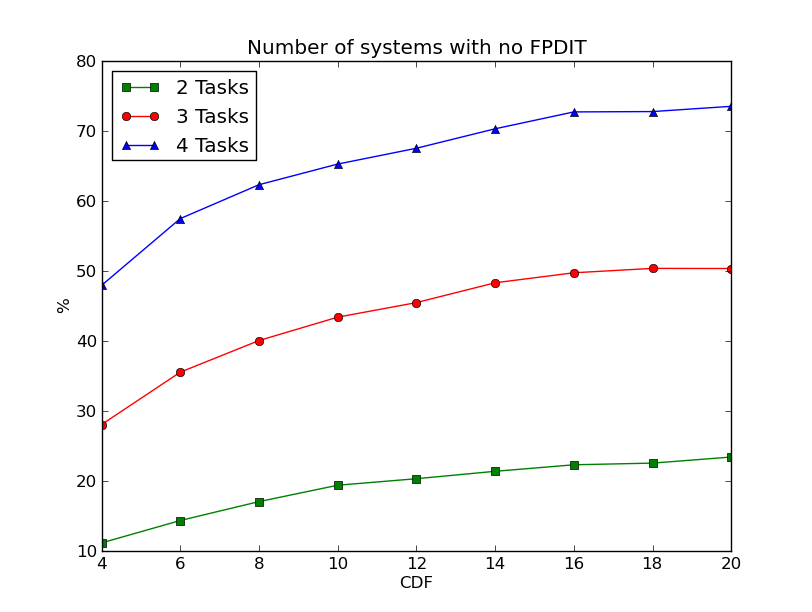
\includegraphics[width=0.5\textwidth]{python-simulation/plots/nofpdit.png}
	\end{center}
	\caption{Evolution of the existence of FPDIT with the CDF}
	\label{fig:noFPDIT}
	\end{figure}

	We observe that the more we are close to the implicit deadline case, the less systems have FPDIT. This is easily explained by the fact that a lower CDF means more idle instant for each task, and thus more opportunities for DITs to happen. Similarly, as all tasks must be synchronized for a DIT to happen, a higher number of tasks results in a decrease in FPDIT density.

\section{C-space of asynchronous systems}
\label{sct:asyncCspace}

	\subsection{Description using DBF}

		The description we presented in Section \ref{sct:cspaceDescr} was general, and
		is thus still relevant. Therefore the C-space is still accurately described by
		the following infinite number of constraints:

		\[
			\sum_{i=0}^{n-1} n_i(t_1, t_2)
			\, C_i \leq t_2 - t_1 \; \forall \: 0 \leq t_1 \leq t_2
		\]

		However, the method used in the synchronous case to remove redundancy does not
		apply here. A more general approach is presented in the following section.

	\subsection{Removing redundancy}

		\subsubsection{Job arrival and deadline}
			Consider an interval $[t_1, t_2]$. If $t_2$ is an instant without any job
			deadline, then by definition the value of $\dbf{t_1, t_2}$ will be equal to
			$\dbf{t_1, t_2^*}$, where $t_2^*$ is the latest deadline before $t_2$.

			A similar argument can be made if $t_1$ is an instant without any job arrival
			(and $t_1^*$ is the earliest arrival after $t_1$). We can thus restricts
			ourselves to intervals where $t_1$ is an instant with at least one job
			arrival, and $t_2$ is an instant with at least one job deadline.

		\subsubsection{Feasibility interval}
			First let us recall how an asynchronous system behaves under an optimal
			scheduler, for example EDF.

			\begin{figure}[h]
				\[
					\begin{array}{r||c|c|c|l}
									& \text{Incomplete} & \text{Transitive} & \text{Stationary} & \cdots \\
						\text{Name} & \text{period} 	& \text{period} 	& \text{period}  	& \\ \hline
						\text{size} & O_{max} 			& H 				& H 				& \cdots \\ \hline
						t \geqslant & 0 				& O_{max} 			& O_{max} + H 		& \cdots
					\end{array}
				\]
				\begin{center}
				\caption{Behavior of an asynchronous system under EDF.}
				\label{fig:asyncBehavior}
				\end{center}
			\end{figure}

As shown in Fig. \ref{fig:asyncBehavior}, the system begins in the \emph{incomplete period}, where all tasks are not in the system. Then, after $O_{max}$ time units, every tasks is in the system and the \emph{transitive period} begins. Then, after $O_{max} + H$ time units, the system is faced with the same pattern of arrival as in $O_{max}$. However, because in $O_{max} + H$ every task is in the system and in $O_{max}$ some were missing, the state of the system will be different. The \emph{stationary period} then begins. It is only after $O_{max} + 2H$ time units that the system comes back into a state in which we can be sure it has been before.

For this reason, as explained in \cite{leung1982complexity}, it is sufficient to check for intervals included in the interval $[O_{max}, O_{max} + 2H]$, which has an exponential length in the number of tasks.

\subsubsection{Using the first periodic DIT}

The FPDIT, if it exists, must occur in the transitive period. Indeed, it cannot occur in the incomplete period by definition ($t_d > O_{max}$) and if it occurred in the $k^{th}$ stationary period, another DIT should have occurred in the transitive period at instant $t_d - k H$ (a contradiction).

As the FPDIT happens when all tasks are in the system, we know that the system will arrive in the exact same state one hyperperiod later ($t_d + H$). We can thus restrict the DBF test to intervals included in the interval $[t_d, t_d + H]$, if the FPDIT exists. This will always be a better interval than $[O_{max}, O_{max} + 2H]$ and if the first periodic DIT does not exist (which can be verified as explained in Section \ref{sct:FPDITexist}), the latter interval can be used.

(Remarque : Avec seulement cette méthode, si un DIT existe on divisera toujours par exactement 4 le nombre de contraintes par rapport à $O_{max} + 2H$)

\subsubsection{Redundancy as an integer linear problem}

The general problem of redundancy of a new linear constraint $C \, X \leq d$ w.r.t. a set of previous linear constraints $A \, X \leq B$ in an ILP can itself be written as the following ILP:

\begin{figure}[h]
$$z = \max C \, X$$
s.t.
\[
\begin{array}{rccc}
  A & X &\leq & B \\
  C & X &\leq & d + 1
\end{array}
\]
with
\[
  \begin{array}{ccc}
    A & : & [n,k] \text{ matrix}\\
    B & : & [n,1] \text{ matrix}\\
    C & : & [n,1] \text{ matrix}\\
    X & : & [1,n] \text{ matrix}\\
    d & : & \text{integer}
  \end{array}
\]
\caption{Redundancy of $CX \leq d$ w.r.t. $A X \leq B$ as an ILP}
\end{figure}

Indeed, if the maximization returns $z=d+1$, it means that there are some integer values accessible with the previous constraints that the new constraint forbids. On the other hands, if the maximization returns $z \leq d$, it means that the limitation expressed in the new constraint is already enforced by the previous constraints. Therefore $z \leq d$ is a necessary and sufficient condition of redundancy of the new constraint.\\

Such a linear problem can be solved by e.g. the simplex algorithm and a branch-and-cut approach. However, in our case the problem is not exactly the same as we have a set of constraints and we want to find all redundant constraints within. A naive method would be to test each constraint against all the others. We present a similar method with an efficient preprocessing when most constraints are redundant in Algorithm \ref{alg:prunRedun}.

\begin{algorithm}
\caption{Removing redundancy from CSPACE}
\label{alg:prunRedun}
  \begin{algorithmic}[1]
    \STATE $CSPACE$ : set of constraints
    \STATE $S \leftarrow \emptyset$
    \STATE \COMMENT{$1^{st}$ pass: test each $cstr$ against previous ones}
    \FOR{$cstr$ \textbf{in} $CSPACE$}
      \IF {$cstr$ is not redundant w.r.t. $S$}
        \STATE $S \leftarrow cstr$
      \ENDIF
    \ENDFOR
    \STATE \COMMENT{$2^{nd}$ pass: test each $cstr$ against every other}
    \FOR{$cstr$ \textbf{in} $S$}
      \STATE Remove $cstr$ from $S$
      \IF {$cstr$ is not redundant w.r.t. $S$}
        \STATE Put $cstr$ back into $S$
      \ENDIF
    \ENDFOR
    \RETURN{S}
  \end{algorithmic}
\end{algorithm}

After doing this, no redundant constraints are left. However, this algorithm takes an exponential time in the number of constraints. An efficient initial description of $CSPACE$, as given by the methods described in previous sections, is therefore preferred.

To summarize, we first reduced the number of constraint from every possible interval $[t_1, t_2]$ to only the interval where $t_1$ is an arrival and $t_2$ is a deadline between $[t_d, t_d + H]$ if $t_d$ exists, or between $[O_{max}, O_{max} + 2H]$ otherwise. After this correct but not efficient description of the C-SPACE, a linear integer approach removes the remaining redundancies.

\section{Numerical Example}

Consider the following task system

    \begin{center}
    \begin{tabular}{|r|c|c|c|c|}
     \hline
      & $O_i$ & $C_i$ & $D_i$ & $T_i$ \\
     \hline
     $\tau_1$ & 8 & $C_1$ & 7 & 15\\
     \hline
     $\tau_2$ & 0 & $C_2$ & 2 & 5\\
     \hline
    \end{tabular}
    \end{center}
    ~\\

The FPDIT happens at $t=15$ and we have $H = 15$. The study interval using the FPDIT is thus $[15, 30]$, which contains 11 intervals $[a,d]$ with $a$ being the arrival of a job, $d$ being the deadline of a job, and $15 \leqslant a < d \leqslant 30$. Those intervals are
$[15, 17]$, $[15, 22]$, $[15, 27]$, $[15, 30]$, $[20, 22]$, $[20, 27]$, $[20, 30]$, $[23, 27]$, $[23, 30]$, $[25, 27]$ and $[25, 30]$. For comparison, the original study interval of $[O_{max}, O_{max} + 2H]$ is $[8, 38]$ which yields 57 intervals.\\

For each $[a, d]$, we have a constraint $$\sum_{i=0}^{n-1} n_i(a, d) \, C_i \leqslant d - a$$ which give a description of the C-space.

We now apply Algorithm \ref{alg:prunRedun} to remove redundancies, leaving us with the following constraints:
$$
\left\{
  \begin{array}{ccccc}
    & & C_2 & \leqslant & 2 \\
    C_1 & + & C_2 & \leqslant & 7
  \end{array}
\right.
$$
The C-space thus contains 11 points $(C_1, C_2) = (1, 1)$, $(2, 1)$, $(3, 1)$, $(4, 1)$, $(5, 1)$, $(6, 1)$, $(1, 2)$, $(2, 2)$, $(3, 2)$, $(4, 2)$ and $(5, 2)$.

Let us now consider the same system but with a synchronous pattern of arrival.

    \begin{center}
    \begin{tabular}{|r|c|c|c|c|}
     \hline
      & $O_i$ & $C_i$ & $D_i$ & $T_i$ \\
     \hline
     $\tau_1$ & 0 & $C_1$ & 7 & 15\\
     \hline
     $\tau_2$ & 0 & $C_2$ & 2 & 5\\
     \hline
    \end{tabular}
    \end{center}

The first DIT happens at time $t_d = 7$. The intervals to consider are thus of the form $[0, t]$ where $t$ is a deadline happening before or at time $t_d$. This yields 2 intervals ($[0, 2]$ and $[0, 7]$) and the following constraints describing the C-space, none of them being redundant:
$$
\left\{
  \begin{array}{ccccc}
    & & C_2 & \leqslant & 2 \\
    C_1 & + & 2 C_2 & \leqslant & 7
  \end{array}
\right.
$$
This time, the C-space only contains 8 points: $(1, 1)$, $(2, 1)$, $(3, 1)$, $(4, 1)$, $(5, 1)$, $(1, 2)$, $(2, 2)$, $(3, 2)$.

Fig. \ref{fig:cspaceComp} shows the two C-spaces in the plane.

\begin{figure}[h]
\begin{center}
  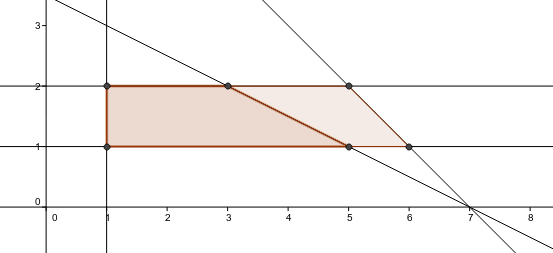
\includegraphics[width=0.5\textwidth]{figs/cspace_example.png}
  \caption{C-space of an asynchronous system and its corresponding synchronous system}
  \label{fig:cspaceComp}
\end{center}
\end{figure}


\section{Experimental C-space size gain of asynchronous systems}
	One of the advantages of asynchronous systems over synchronous systems in the
	context of periodic tasks is that the critical instants of asynchronous systems
	cannot be more constraining for the C-space than synchronous instants. For this
	reason, it has long been known that modifying task offsets when possible during
	the design of a real-time system is a useful trick to fit a heavy but periodic task set
	into a given platform.
	
	In Fig.~\ref{fig:sizeRatio} a number of feasible asynchronous task sets without
	synchronous instants were generated and the size of their C-space was
	calculated and compared with the size of the C-space of the same
	task sets with all task offsets set to zero. In other words, this figure
	evaluates the feasibility gain of adding random offsets to a synchronous task
	set. It is assumed that a more advanced strategy to assign these offsets
	would yield a greater difference.
	
	\begin{figure}[h]
		\begin{center}
			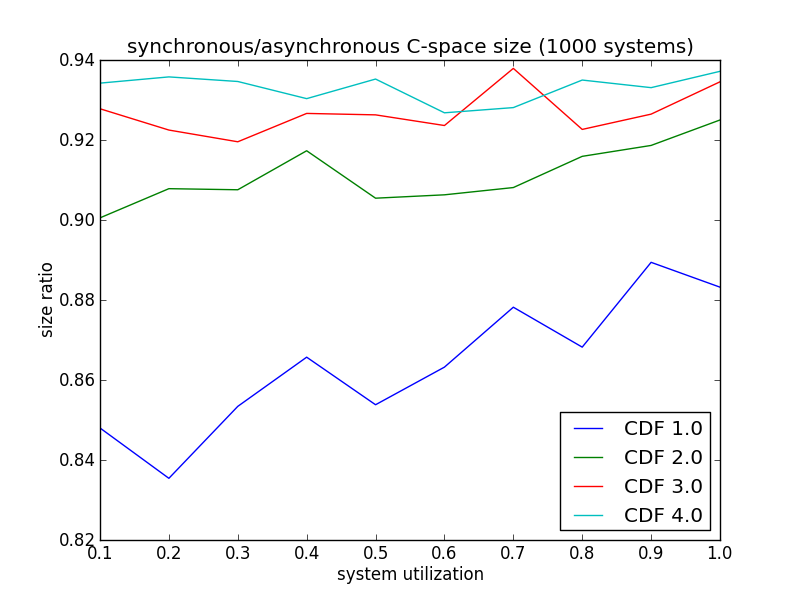
\includegraphics[width=0.5\textwidth]{figs/sizeRatio.png}
			\caption{C-space size ratio between asynchronous and equivalent synchronous
			systems}
			\label{fig:sizeRatio}
		\end{center}
	\end{figure}
	
	
\section{Conclusion}


% conference papers do not normally have an appendix


% use section* for acknowledgement
% \section*{Acknowledgment}


% The authors would like to thank...





% trigger a \newpage just before the given reference
% number - used to balance the columns on the last page
% adjust value as needed - may need to be readjusted if
% the document is modified later
%\IEEEtriggeratref{8}
% The "triggered" command can be changed if desired:
%\IEEEtriggercmd{\enlargethispage{-5in}}

% references section

% can use a bibliography generated by BibTeX as a .bbl file
% BibTeX documentation can be easily obtained at:
% http://www.ctan.org/tex-archive/biblio/bibtex/contrib/doc/
% The IEEEtran BibTeX style support page is at:
% http://www.michaelshell.org/tex/ieeetran/bibtex/
%\bibliographystyle{IEEEtran}
% argument is your BibTeX string definitions and bibliography database(s)
%\bibliography{IEEEabrv,../bib/paper}
%
% <OR> manually copy in the resultant .bbl file
% set second argument of \begin to the number of references
% (used to reserve space for the reference number labels box)
% \nocite{*}
\bibliographystyle{plain}
\bibliography{dit-paper}





% that's all folks
\end{document}


